\section{Тема лабораторной  работы}
Лабораторная работа посвящена разбору следующих структур данных: деревья, пирамида или двоичная куча, очередь с приоритетами, а также пирамидальной сортировке - еще одному виду сортировки за время \eqref{eq:eql}
\begin{equation}
    \centering
    \label{eq:eql}
    T(n) = T1(n) + T2(n) = O(n\log(n)).
\end{equation}


\section{Определение}
\textbf{Неубывающая пирамида} -  это почти полное дерево (только уровень листьев может быть неполным), удовлетворяющее требованию – ключ каждой вершины не больше ключа родителя. Аналогично определяются невозрастающие пирамиды.

\cite{algorithms_1, algorithms_2}

\section{Задача№1:Неубывающая пирамида}
Структуру данных «куча», или, более конкретно, «неубывающая пирамида», можно реализовать на основе массива.
Для этого должно выполнятся основное свойство неубывающей пирамиды, которое заключается в том, что для каждого 1 <= i <= n выполняются условия:

\begin{itemize}

\item если 2i <= n, то ai <= a2i,
\item если 2i + 1 <= n, то ai <= a2i+1.

\end{itemize}
Дан массив целых чисел. Определите, является ли он неубывающей пирамидой.
 \begin{itemize}
    \item \textbf{Формат входного файла (input.txt)}.Первая строка входного файла содержит целое число n (1 <= n <= 106). Вторая строка содержит n целых чисел, по модулю не превосходящих 2 * 109.
    \item \textbf{Формат выходного файла (output.txt)}. Выведите «YES», если массив является неубывающей пирамидой, и «NO» в противном случае.
	\item Ограничение по времени. 2 сек.
    \item Ограничение по памяти. 256 мб.
\end{itemize}

\begin{table}[H]
	\caption{Примеры входных и выходных файлов}
	\begin{center}
		\begin{tabular}{|l|c|r|}
			\hline
			    № & input.txt & output.txt \\ \hline
			1 & 1 0 1 2 0 & NO \\ \hline
                2 & 1 3 2 5 4 & YES \\ \hline
		\end{tabular}
		\label{tabular:tab_examp_2}
	\end{center}
\end{table}


\newpage
\section{Решение}

\subsection{Листинг кода}
\begin{code}
	\inputminted[breaklines=true, xleftmargin=1em, linenos, frame=single, framesep=10pt, fontsize=\footnotesize, firstline=1, lastline=16]{haskell}{listings/1.py}
	\caption{Код задачи №1}
\end{code}

\subsection{Текстовое объяснение решения задачи}
Данная задача позволяет на самом простом примере разобраться с таким типом данных как куча или же неубывающая пирамида. При помощи функции необходимо проверить верность равенства, данного в тексте задачи и вывести в output файл слова “YES” или “NO” в зависимости от результата выполнения кода.


\subsection{Результат работы кода на примере из текста задачи}

\begin{figure}[H]
    \begin{center}
		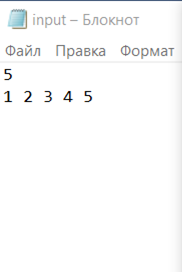
\includegraphics[scale=0.6]{input}
		\caption{Input file}
		\label{pic:pic_name} % название для ссылок внутри кода
  \end{center}
  \begin{center}
		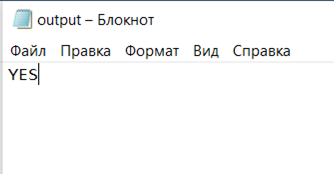
\includegraphics[scale=0.7]{output}
		\caption{Output file}
		\label{pic:pic_name} % название для ссылок внутри кода
  \end{center}
\end{figure}

\newpage
\section*{Вывод}
в лабораторной работе я встретилась с понятиями кучи и очереди с приоритетами, разобралась в их взаимосвязи и рассмотрела разные варианты реализации подобных кодов.
\addcontentsline{toc}{section}{Вывод}